%!/usr/bin/env pdflatex
%-*- coding: utf-8 -*-
%@author : Romain Graux
%@date : 2022 June 07, 17:49:15
%@last modified : 2022 June 16, 16:14:49

\label{sec:performance}


\section{Visual performance}

Now that we have a fully working model, it is time to evaluate its performance. On the Figure~\ref{fig:mitch-all}, we can see the impact of the span value on the distortion of the \textit{mitch} point cloud with a voxelized depth of $8$, which corrresponds to a voxelized point cloud of size $256 \times 256 \times 256$. 
The whole point cloud has been partitioned into $64 \times 64 \times 64$ smaller point clouds, which have been fed to the analysis transform.

\begin{figure}
    \centering
    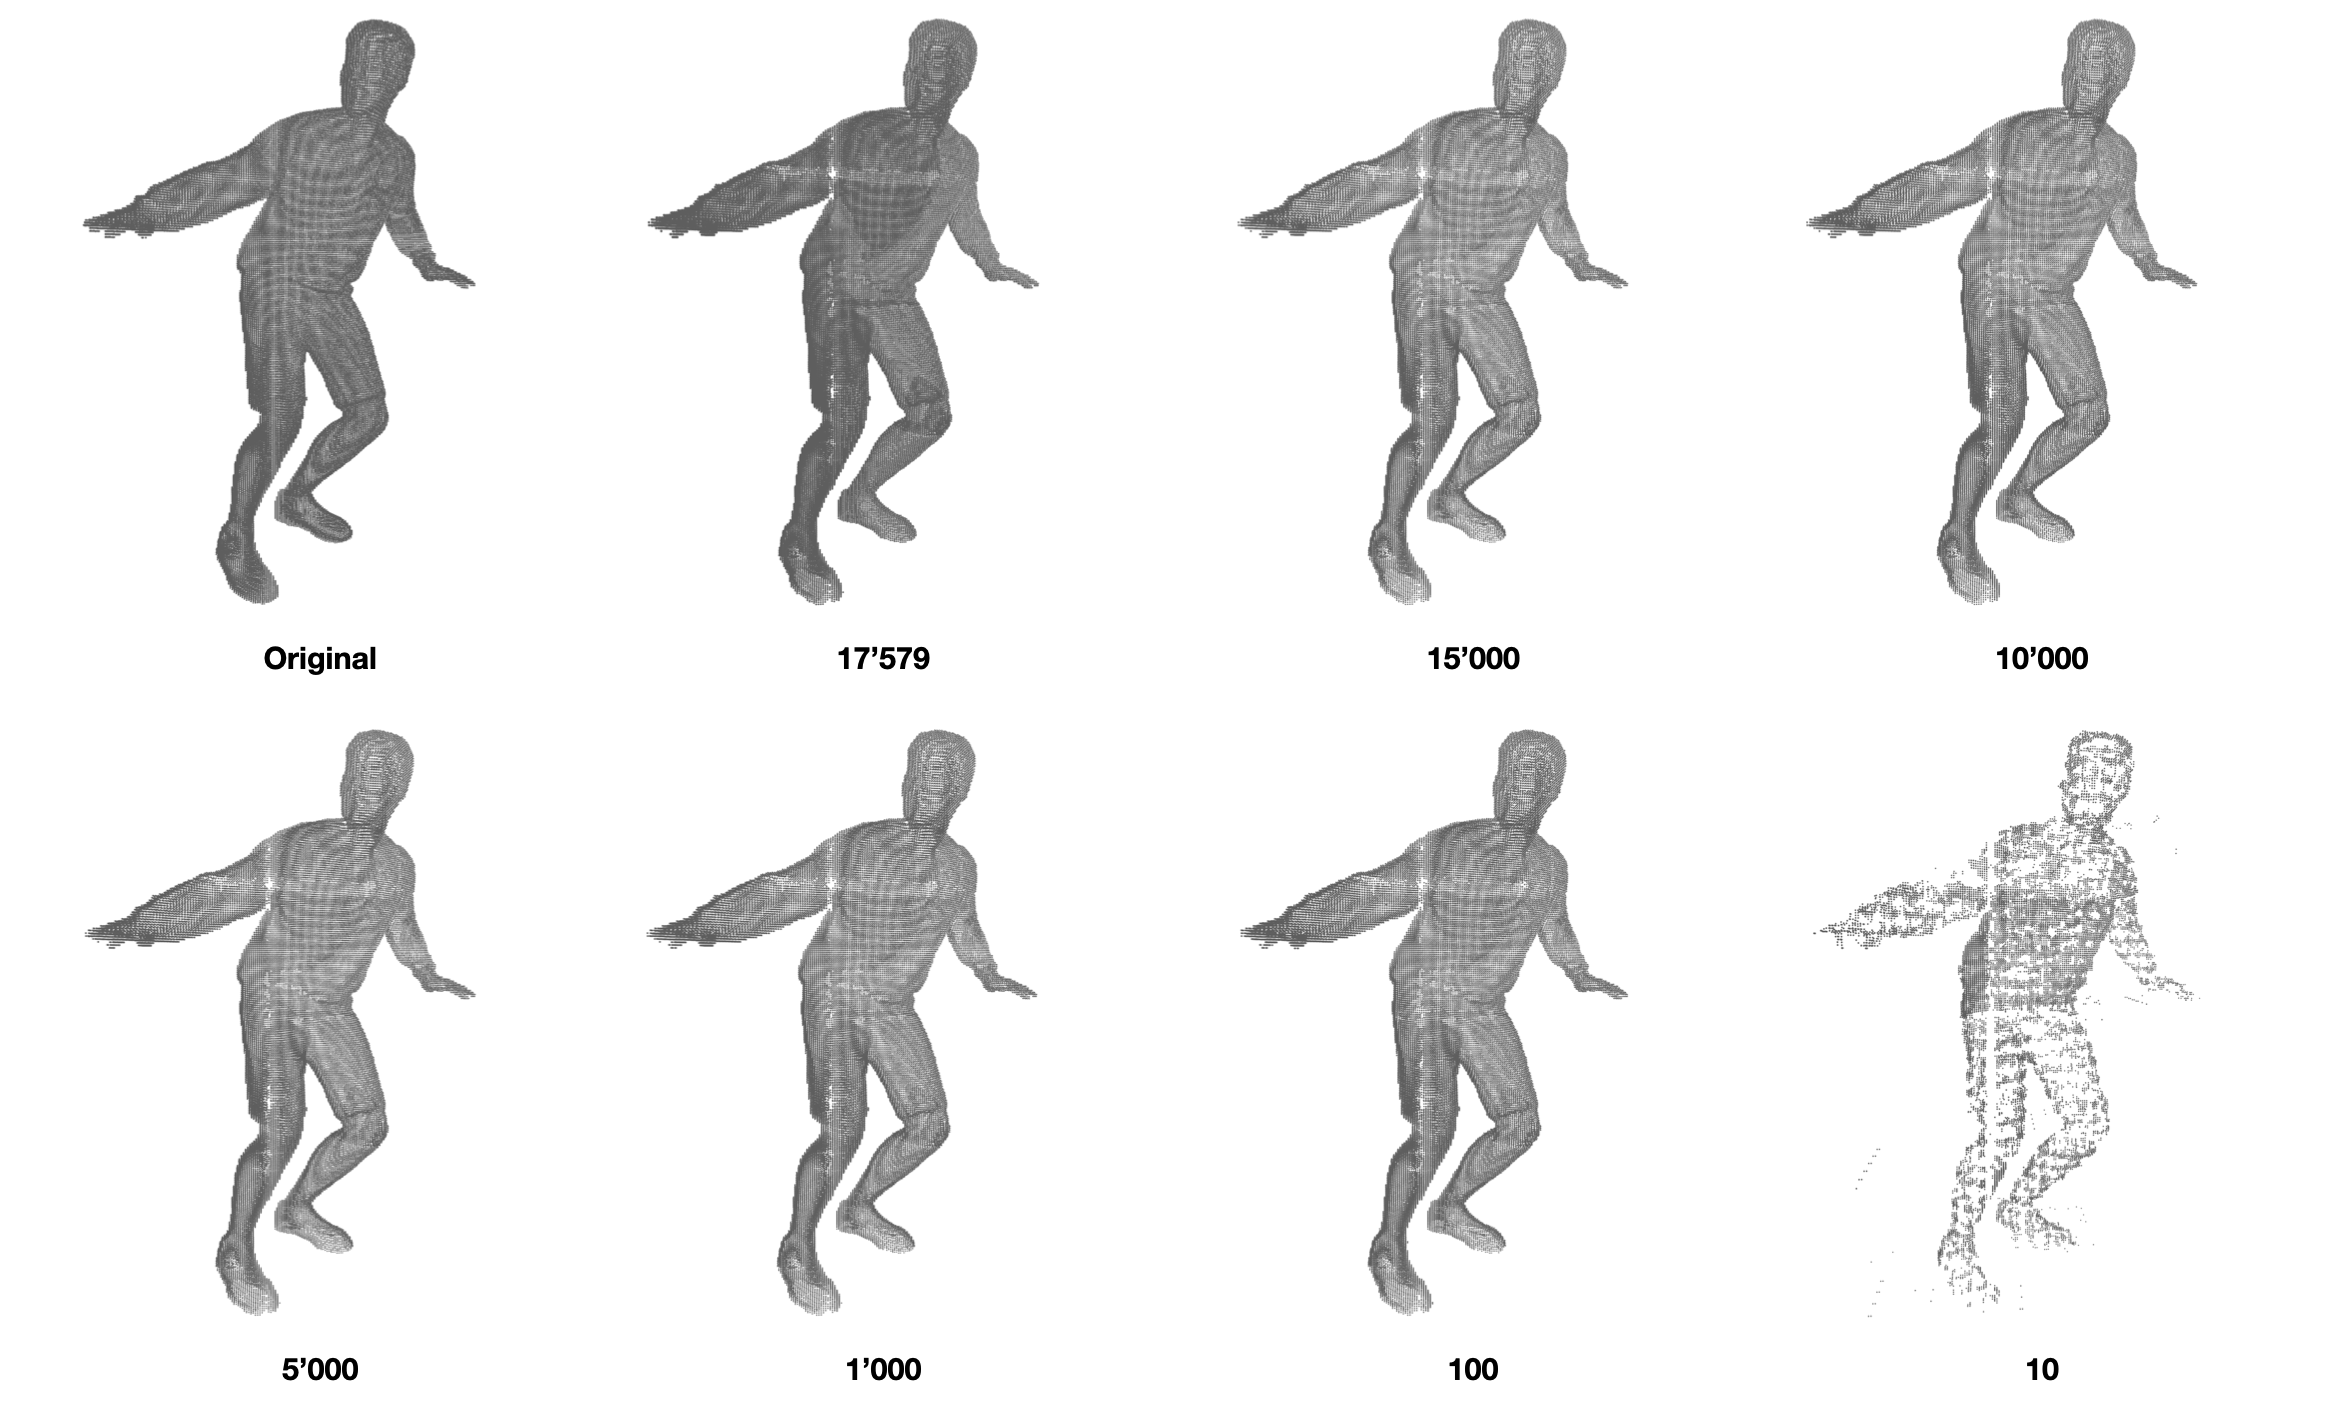
\includegraphics[width=0.9\textwidth]{mesh/all/mitch/results_}
    \caption{Mitch point cloud distortion regarding the span value with a voxelized depth of $8$}
    \label{fig:mitch-all}
\end{figure}

\section{Rate-distortion analysis}

\begin{figure}
    \centering
    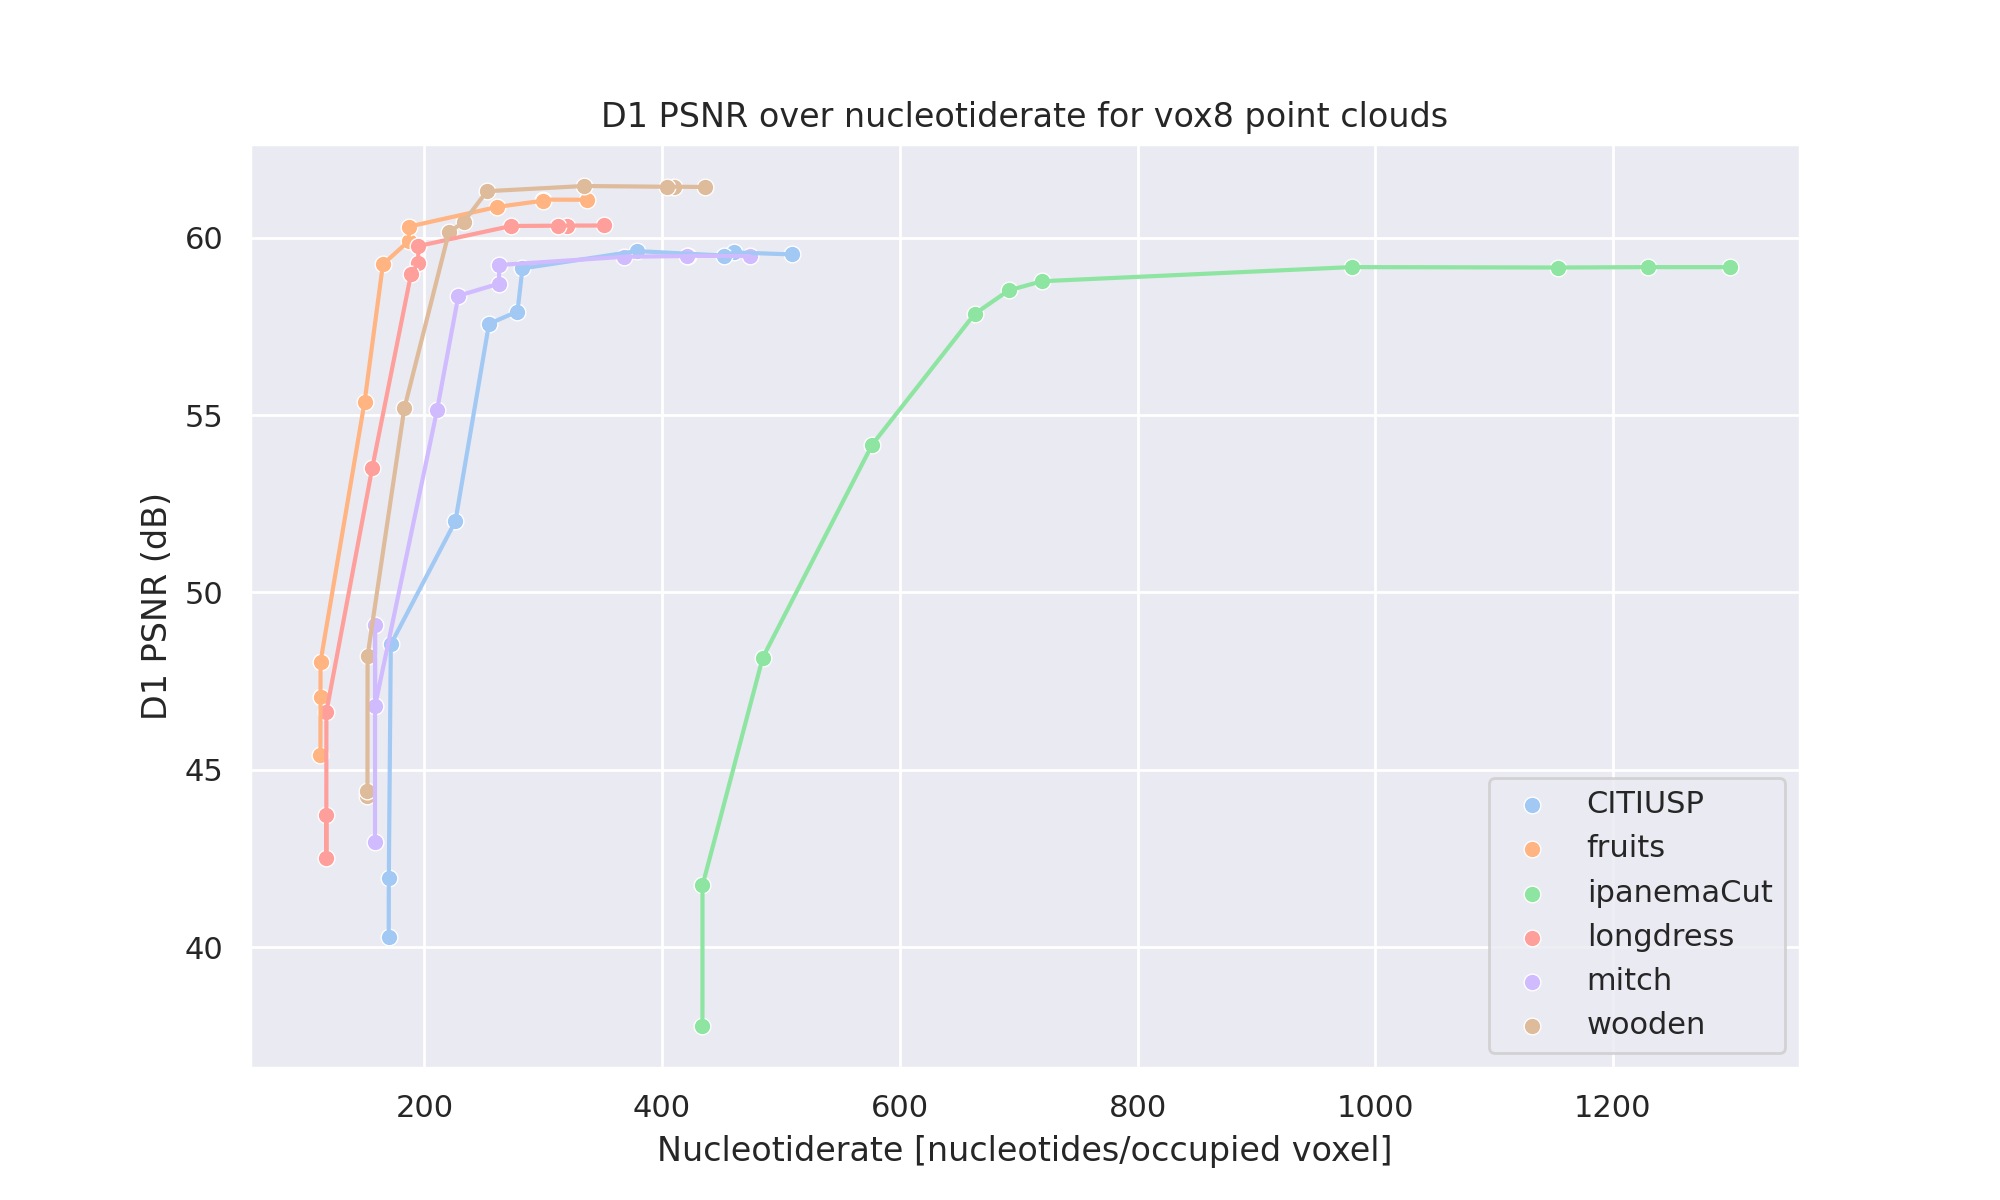
\includegraphics[width=0.9\textwidth]{rate_distortion_span_full2}
    \caption{Rate-distortion analysis regarding the nucleotiderate (controlled by the span value)}
    \label{fig:rate-distortion}
\end{figure}

As we can see in the Figure~\ref{fig:rate-distortion}, the rate-distortion can be easily controlled by the span value. 

These specific nucleotiderates have been computed for the following span values: $$\text{span values} \in \{5, 7, 10, 20, 40, 50, 100, 1000, 5000, 10000, 17579\}$$
We see that the two first span values end up with the same nucleotide rate, while the distortion is much lower for the span value of $7$. We also see that the PSNR is rising quite quickly for the first values without impacting the nucleotide rate much. Both can be explained by the codewords lengths that are small for the first codebooks ($2$ and $3$ codewords lengths) and especially for the span value of $7$, it has $2$ coefficients ($6$ and $7$) that are encoded on length $3$ codewords while the rest is encoded on length $2$ codewords (because falling in the first category codebook). So if the frequency of the $2$ coefficients is not too high, it does not change the final stream length and as we see in the Figure~\ref{fig:quantized-y-1000}, the distribution of the latent representation is not concentrated close to the minimum or the maximum value so there will not be too many extreme values encoded in the final stream.

Weirdly, the ipanemaCut~\ref{fig:ipanema-cut} shows a much higher nucleotide rate than all the others point clouds, it could be explained by the number of occupied voxels that are quite low compared to the overall number of voxels. But the CITIUSP~\ref{fig:citiusp} has a similar structure and has a better nucleotide rate over distortion ratio.

Finally, we can observe that we obtain a maximum PSNR around $60$ quite quickly and that it is no longer increasing with a higher nucleotide rate. It can be explained by the linear quantization that is the only lossy part of the algorithm. Since the distribution of the latent reprsentation is non uniform, as seen on Figure~\ref{fig:quantized-y-1000}, it can explain why the quantization is sub-optimal to turn continuous values into discrete ones.

\section{DNA storage simulation}

\tocontinue{}
